\documentclass[11pt,a4paper,twoside]{memoir}
\usepackage[final,protrusion,babel]{microtype}
\usepackage[T1]{fontenc}
\usepackage[utf8]{inputenc}

\newcommand{\longtitle}{Automatic Graph Tracking in Probabilistic Programs via Source Transformations}

% LINKS AND PDF OPTIONS
\usepackage[pdfa,final]{hyperref}
\hypersetup{
  pdfinfo={
    Author={Philipp Gabler},
    Title={\longtitle}
  },
  hyperfootnotes=false
}

\usepackage{typographic_setup}

\usepackage[english]{babel}
\usepackage[style=english]{csquotes}
% \usepackage{xspace}
\usepackage[final]{graphicx}
\usepackage[textsize=tiny]{todonotes}

% \usepackage[originalcommands]{ragged2e} % improved ragged paragraphs in abstract
\usepackage{eso-pic}

% \usepackage{commath}
% \usepackage{amsmath}
% \usepackage{amssymb}
% \usepackage{MnSymbol} % incompatible with amssymb and amsfonts
% \usepackage{mathtools} % improvements on amsmath
%\usepackage{pifont}
% \usepackage{fourier-orns}

% \usepackage[final]{mylistings}
\usepackage[final]{listings}
\usepackage[charsperline=94, usebox=false, usecolors=false]{jlcode}


%-------------------------------------------------------------------------------
% BIBLATEX
%

\usepackage[%
  backend=biber,
  citestyle=authoryear-comp,
  style=authoryear,
  sortcites=true,
  sorting=nyt,
  %natbib=true,
  giveninits=true,
  url=false,
  isbn=false,
  date=year,
  urldate=ymd
]{biblatex}
\DeclareNameAlias{default}{last-first}

% only capitalize real titles
% http://tex.stackexchange.com/a/22981/46356
% \DeclareFieldFormat{sentencecase}{\MakeSentenceCase{#1}}
% \renewbibmacro*{title}{%
%   \ifthenelse{\iffieldundef{title}\AND\iffieldundef{subtitle}}
%     {}
%     {\printtext[title]{%
%         \printfield[sentencecase]{title}%
%         \setunit{\subtitlepunct}%
%         \printfield[sentencecase]{subtitle}}
%       \newunit}%
%   \printfield{titleaddon}}

\defbibheading{memoir}[\bibname]{\chapter*{#1}}
\setcounter{biburllcpenalty}{7000}
\setcounter{biburlucpenalty}{8000}

\AtEveryBibitem{\clearlist{language}} % clears language
\AtEveryBibitem{\clearlist{pagetotal}} % clears book pages
\renewcommand*\bibnamedash{\rule[0.48ex]{3em}{0.14ex}\space}
\renewcommand*{\multinamedelim}{,\space}
\renewcommand*{\finalnamedelim}{\space\&\space}

\addbibresource{refs.bib}

%-------------------------------------------------------------------------------
% OTHER SETTINGS
%

% toc
% \setlength{\cftbeforechapterskip}{1ex} % decrease space between sections

% floats
\newlength{\capwidth}
\addtolength{\capwidth}{\textwidth}
\addtolength{\capwidth}{-4ex}
\captionwidth{\capwidth}
\captionstyle[\raggedright]{}
% \renewcommand{\textfloatsep}{\baselineskip}

\newsubfloat{figure}
\subcaptionfont{\sffamily}

\setFloatBlockFor{section} % like \usepackage[section]{placeins}, but from memoir


% listing floats
\newfloat[chapter]{lstfloat}{lolst}{Listing}
\newsubfloat{lstfloat}
\lstdefinestyle{lstfloat}{%
  aboveskip=\smallskipamount,
  belowskip=\smallskipamount,
  frame=tb,
  rulecolor=\color{black},
}

% algorithm floats
\usepackage{algpseudocode}
\algrenewcommand\textproc{\texttt}
\algnewcommand{\LineComment}[1]{\State \(\triangleright\) \textit{#1}}

\newcommand{\algorithmname}{Algorithm}
\newcommand{\listalgorithmname}{List of Algorithms}
\newlistof{listofalgorithms}{loa}{\listalgorithmname}
\newfloat[chapter]{algorithm}{loa}{\algorithmname}
\newfixedcaption{\falgcaption}{algorithm}
\newlistentry{algorithm}{loa}{0}


% \usepackage{float}
% \floatstyle{ruled}
% \restylefloat{algorithm}

% epigraphs
\setlength{\epigraphwidth}{\textwidth}
\setlength{\epigraphrule}{0pt}

% \setcounter{topnumber}{1}       % allow only one float per page

% no need for colors here...
% \colorlet{textred}{darkgray!80}
% \colorlet{textblue}{darkgray!80}

% \newcommand{\lstlistingautorefname}{Listing}

% csquotes blockquote
% redefine spacing above/below; hacking original latex definition from 
% http://mirrors.ctan.org/macros/latex/base/classes.dtx
\makeatletter
\newenvironment{myblockquote}
               {\vspace{-1em}\list{}{\listparindent 1.5em%
                        \itemindent    \listparindent
                        \rightmargin   \leftmargin
                        \parsep        \z@ \@plus\p@}%
                \item\relax}
               {\endlist\vspace{-0.5\baselineskip}}
\makeatother
\SetBlockEnvironment{myblockquote}


% TIKZ SETUP
% \usepackage{tikz}
% \usepackage{rotating}


%-------------------------------------------------------------------------------
% DOCUMENT MACROS
%
\newcommand{\ie}{i.e.\xspace}
\newcommand{\eg}{e.g.\xspace}
\newcommand{\cf}{cf.\xspace}
\newcommand{\margintodo}[1]{\todo[noline, size=\tiny]{#1}}
% \newcommand{\CC}{{C\nolinebreak[4]\hspace{-.05em}\raisebox{.22ex}{\small\textbf{++}}}}
% \newcommand{\autosubref}[1]{{\hyperref[#1]{Subsection~\ref*{#1}~--~\nameref*{#1}}}}
% \newcommand{\autosubref}[1]{\autoref{#1}}
% \newcommand{\aref}[1]{\hyperref[#1]{Appendix~\ref{#1}}}
\newcommand{\mathlst}[1]{\text{\lstinline|1|}}


% MATH STUFF
\newcommand{\iid}{i.i.d.}
\newcommand{\prob}[2][\empty]{{p}_{#1}(#2)}
\newcommand{\Prob}[1]{\mathbb{P}[#1]}
\newcommand{\Exp}[2][\empty]{\mathbb{E}_{\ifx#1\empty\empty\else{\! #1}\fi}[#2]}
\newcommand{\Var}[2][\empty]{\mathbb{V}_{\ifx#1\empty\empty\else{\! #1}\fi}[#2]}
\newcommand{\Expd}[2][\empty]{\mathbb{E}_{\ifx#1\empty\empty\else{\! #1}\fi}\!\left[#2\right]}
\newcommand{\Vard}[2][\empty]{\mathbb{V}_{\ifx#1\empty\empty\else{\! #1}\fi}\left[#2\right]}
\newcommand{\entropy}[1]{\mathrm{H}(#1)}
\newcommand\given[1][]{\:#1\vert\:}
\newcommand{\distr}[1]{\mathrm{#1}}
\newcommand{\from}{\sim}
\newcommand{\iidfrom}{\stackrel{\text{iid}}{\sim}}
\newcommand{\kldiv}[2]{\mathrm{D}_{\text{KL}}(#1 \parallel #2)}
\newcommand{\transpose}[1]{#1^{\mathrm{T}}}
\newcommand{\inverse}[1]{#1^{-1}}
\newcommand{\RR}{\mathbb{R}}
\newcommand{\NN}{\mathbb{N}}
\newcommand{\ZZ}{\mathbb{Z}}
\newcommand{\Sqrt}[1]{#1^{\frac{1}{2}}}
\newcommand{\kth}[2][k]{#2^{(#1)}}
\newcommand{\sequence}[2][k \ge 1]{(#2)_{#1}}
\newcommand{\indicator}[1]{\vvmathbb{1}(#1)}
\newcommand{\Normal}{\distr{Normal}}
\newcommand{\MVNormal}{\distr{MvNormal}}
\newcommand{\vect}[1]{\boldsymbol{#1}}
\newcommand{\Likelihood}[1]{\mathcal{L}(#1)}
\newcommand{\Loglikelihood}[1]{\ell(#1)}
\newcommand{\Dif}{\mathop{}\!\mathrm{D}}
\newcommand{\CoDif}{\mathop{}\!\mathrm{D}^{*}}
\newcommand{\dif}{\mathop{}\!\mathrm{d}}
\newcommand{\envert}[1]{\left\lvert#1\right\rvert}
\newcommand{\enVert}[1]{\left\lVert#1\right\rVert}
\DeclareMathOperator{\diag}{diag}
\DeclareMathOperator*{\argmin}{arg min}
\DeclareMathOperator{\Span}{span}
\DeclareMathOperator{\proj}{proj}
\DeclareMathOperator{\card}{card}
\DeclareMathOperator{\tr}{tr}
\DeclareMathOperator{\rank}{rank}
\DeclareMathOperator{\sgn}{sgn}
\DeclareMathOperator{\supp}{supp}
\DeclareMathOperator{\ident}{id}

% Broadcast syntax for math mode, from https://tex.stackexchange.com/a/490779/46356
\makeatletter
\DeclareRobustCommand{\broadcast}[1]{%
  \begingroup
  \binrel@{#1}%
  \ifx\binrel@@\mathbin \mathbin{.{#1}}\else
  \ifx\binrel@@\mathrel \mathrel{.}#1\else
  \phg@ordop{#1}\fi\fi
  \endgroup
}
\def\phg@ordop#1{%
  \sbox\z@{\thinmuskip=0mu$#1a$}%
  \sbox\tw@{\thinmuskip=1000mu$#1a$}%
  \ifdim\wd\tw@>\wd\z@
    % operator
    \mathop{{#1}.}%
  \else
    #1.
  \fi
}
\makeatother

\newcommand{\juliapackage}[1]{\href{https://github.com/search?q=#1&type=Repositories}{\texttt{#1}}}
\newcommand{\turingjl}{\juliapackage{Turing.jl}}
\newcommand{\irtrackerjl}{\juliapackage{IRTracker.jl}}
\newcommand{\autogibbsjl}{\juliapackage{AutoGibbs.jl}}
\newcommand{\dppljl}{\juliapackage{DynamicPPL.jl}}


%-------------------------------------------------------------------------------
% DOCUMENT
% -------------------------------------------------------------------------------
\title{\longtitle}

% \includeonly{background}

\begin{document}
\chapterstyle{hangnum}
\pagestyle{plain}
\frontmatter

\setcounter{page}{1} % titling page resets to 1 afterwards
%%%% Time-stamp: <2015-04-05 11:32:08 vk>
%% ========================================================================
%%%% Disclaimer
%% ========================================================================
%%
%% created by
%%
%%      Stefan Kroboth and Karl Voit
%%
%% this title page fulfills the requirements of the corporate design
%% of Graz University of Technology (correct placement of logo)

\begin{titlingpage}

%\large  %% basic font size of the titlepage

%% placing the TU Graz logo exactly as Corporate Design demands:
%%   40mm of Logo (here: 2mm margin in picture!)
%%    8mm from top and from right
%% Source: http://portal.tugraz.at/portal/page/portal/TU_Graz/Services/BDR/Oeffentlichkeitsarbeit/CD/Logo%20Anwendungsrichtlinien
\AddToShipoutPicture*{%
  \AtPageUpperLeft{%
    \hspace{\paperwidth}%
    \raisebox{-19mm}{%\baselineskip}{%
     \makebox[-4mm][r]{\includegraphics[width=42mm]{figures/TU_Graz_Logo.pdf}}
}}}%

\begin{center}
~
\vfill\vfill\vfill

\sffamily

Philipp Gabler, BSc

\vfill

{\LARGE\bfseries sldfk sldkf}

{\large\bfseries sldkf sldf}

\vfill\vfill\vfill\vfill

{\normalsize\bfseries Masterarbeit}\\
\vfill
zur Erlangung des akademischen Grades\\
{Master of Science}\\
\vfill
eingereicht an der\\
{\normalsize\bfseries Technischen Universität Graz}

\vfill\vfill\vfill
\vfill\vfill\vfill

Betreuer\\
Univ.-Prof. Dipl.-Ing. Dr.\thinspace{}mont. Franz Pernkopf\\
\vfill
Mitbetreuer\\
Martin Trapp\\
\vfill
\vfill
Institut für Signalverarbeitung und Sprachkommunikation\\

\vfill

Fakultät für Informatik und Biomedizinische Technik

\vfill\vfill\vfill

{\scriptsize Graz, XXXX~2020}

\end{center}
\end{titlingpage}

%% end of title page
%%% Local Variables:
%%% mode: latex
%%% TeX-master: "main"
%%% End:

\setcounter{page}{3}

\cleartorecto
\epigraph{%
  Es macht so glücklich, Computer zu sein:\\
  alle Schererein\\
  verwandeln sich in Rechnerei\\
  und gehn in Millionstel Sekunden vorbei.\\
  In wenigen \enquote{bit}\\
  kriegst du die ganze Weltordnung mit\\
  im Grund\\
  heißt die Frage ja immer \enquote{Sein oder Nichtsein},\\
  die erledigst du sogar ohne Und,\\
  den ganzen Moder\\
  mit einem einzigen Oder.
}{\textit{Andreas Okopenko}}

\cleartorecto
%%%% Time-stamp: <2017-02-14 16:01:12 vk>
%% ========================================================================
%%%% Disclaimer
%% ========================================================================
%%
%% created by
%%
%%      Karl Voit, and Matthias Wölbitsch
%%
%%
%% code for the date and signature fields adapted from
%% http://tex.stackexchange.com/a/20562


\newcommand{\textfield}[2]{
  \vbox{
    \hsize=#1\kern3cm\hrule\kern1ex
    \hbox to \hsize{\strut\hfil\footnotesize#2\hfil}
  }
}


\section*{Affidavit}
I declare that I have authored this thesis independently, that I have
not used other than the declared sources/resources, and that I have
explicitly indicated all material which has been quoted either
literally or by content from the sources used. The text document
uploaded to \abbrev{TUGRAZ}online is identical to the present master‘s
thesis.

\hbox to \hsize{\textfield{4cm}{Date}\hfil\hfil\textfield{7cm}{Signature}}



%%% Local Variables:
%%% mode: latex
%%% TeX-master: "main"
%%% End:


\cleartorecto
\begin{adjustwidth}{\absleftindent}{\absrightindent}
  \phantomsection
  \label{license}
  \currentpdfbookmark{License}{license}

  \begin{symbolicfootnotes}
    \abstracttextfont
    \vspace*{\stretch{1}}
    \begin{center}
      This work is licensed under a \\ \href{http://creativecommons.org/licenses/by-sa/4.0/}{Creative
        Commons Attribution-ShareAlike 4.0 International License}.
    \end{center}
    \begin{center}
      \includegraphics[scale=1]{figures/by-sa}
    \end{center}
    \vspace{\stretch{2}}
    \begin{center}
      All code samples, unless otherwise noted or cited from other sources, \\ are also available under an
      \href{http://opensource.org/licenses/MIT}{\abbrev{MIT} license}:
    \end{center}
    \vspace*{-1ex}
    \begin{ttfamily}
      \setlength{\parskip}{12pt}
      \setlength{\parindent}{0pt}
      The MIT License (MIT)

      Copyright (c) 2020 Philipp Gabler

      Permission is hereby granted, free of charge, to any person obtaining a copy of this software
      and associated documentation files (the "Software"), to deal in the Software without
      restriction, including without limitation the rights to use, copy, modify, merge, publish,
      distribute, sublicense, and/or sell copies of the Software, and to permit persons to whom the
      Software is furnished to do so, subject to the following conditions:

      The above copyright notice and this permission notice shall be included in all copies or
      substantial portions of the Software.

      THE SOFTWARE IS PROVIDED "AS IS", WITHOUT WARRANTY OF ANY KIND, EXPRESS OR IMPLIED, INCLUDING
      BUT NOT LIMITED TO THE WARRANTIES OF MERCHANTABILITY, FITNESS FOR A PARTICULAR PURPOSE AND
      NON\-IN\-FRINGE\-MENT. IN NO EVENT SHALL THE AUTHORS OR COPYRIGHT HOLDERS BE LIABLE FOR ANY
      CLAIM, DAMAGES OR OTHER LIABILITY, WHETHER IN AN ACTION OF CONTRACT, TORT OR OTHERWISE, ARISING
      FROM, OUT OF OR IN CONNECTION WITH THE SOFTWARE OR THE USE OR OTHER DEALINGS IN THE SOFTWARE.
    \end{ttfamily}
    
    \vspace{2ex}
    
    \begin{adjustwidth}{0.5\absleftindent}{0.5\absrightindent}
      \begin{center}
        % A full |sbt| project containing many of the code samples can be found at
        % \url{https://github.com/phipsgabler/dsl-examples}. 

        The \LaTeX{} source of this document is available at\\
        \url{https://github.com/phipsgabler/master-thesis} \\
        or upon request from the author\footnote{\texttt{pgabler@student.tugraz.at}}.
      \end{center}
    \end{adjustwidth}
    
    \vspace{\stretch{1}}
  \end{symbolicfootnotes}
\end{adjustwidth}


%%% Local Variables: 
%%% TeX-master: "main"
%%% End:


%-------------------------------------------------------------------------------
% ABSTRACT
\cleartorecto
\renewcommand{\abstractname}{Abstract}
\begin{abstract}
  \phantomsection
  \label{abstract}
  \currentpdfbookmark{Abstract}{abstract}
  
  \noindent Probabilistic programming is a means of describing stochastic models through the syntax
  of a programming language.  These models describe probability distributions as stochastic
  function.  Probabilistic programms distinguish themselves from normal programs by the possibility
  of being sampled from conditionally, with some of the internally variables fixed to observed
  values.  While probabilistic programming systems are often implemented as separate,
  domain-specific languages, they can also be embedded into \enquote{host} programming languages
  with sufficient syntactic flexibility.  The latter is advantageous if one wants to use regular
  general-purpose programming constructs or interact with other functionalities of the host
  language.

  This thesis first presents a general system for extracting rich computation graphs in the Julia
  programming language.  These graphs contain the whole recursive structure of a program in terms of
  executed instructions of the intermediate representation used by the compiler.  The system is
  flexible enough to be used for multiple purposes that require dynamic program analysis or abstract
  interpretation, such as automatic differentiation or dependency analysis.

  The second contribution is the application of the described graph tracking system to programs
  written for Turing, a probabilistic programming system implemented as an embedded language within
  Julia.  The functions describing a Turing model can be analyzed, and from them the dependency
  structure of involved random variables be extracted.  Given this structure, analytical Gibbs
  conditionals can be calculated and passed to Turing's inference mechanism, where they are used in
  Markov-Chain Monte Carlo samplers approximating the modelled distribution.
\end{abstract}

%%% Local Variables:
%%% mode: latex
%%% TeX-master: "main"
%%% End:

\chapter*{Acknowledgements}
\label{cha:notation}
% \addcontentsline{toc}{chapter}{Acknowledgements}
\phantomsection
\label{acknowledgements}
\currentpdfbookmark{Acknowledgements}{acknowledgements}

\noindent Better late than never.  I owe great thanks to:
\begin{itemize}
\item Martin Trapp, for neverlasting encouragement and help;
\item Franz Pernkopf, for all the freedom;
\item Hong Ge \& the Turing Team, for giving my work a basis and meaning; 
\item the Julia Community, for making all the work possible;
\item the best of all parents, for their unbounded support.
\end{itemize}


%%% Local Variables: 
%%% TeX-master: "main"
%%% End:

%-------------------------------------------------------------------------------
% TOC
\cleartorecto
\begingroup
\hypersetup{hyperindex=true}
\label{toc}
\currentpdfbookmark{Contents}{toc}
\tableofcontents*
\endgroup

\chapter*{Notation}
\label{cha:notation}
\addcontentsline{toc}{chapter}{Notation}
% \currentpdfbookmark{Notation}{notation}

\begin{description}[style=nextline, leftmargin=4cm]
\item[\(\Prob{\Theta \in A \given X = x}\)] Random variables and their realizations will usually be
  denoted with upper and lower case letters, respectively
  (with some exceptions for Greek variable names).  Sets
  are written with uppercase letters.
\item[{\(\Exp{X}, \Var[X]{f(X, Y)}\)}] Expectation and variance; if necessary, the variable with
  respect to which the moment is taken is indicated.
\item[\(\phi(x), f_{Z}(x)\)] Density functions are named using letters commonly used for functions,
  with an optional subscript indicating the random variable they belong to.  Densities always come
  with implied base measures depending on the type of the random variable.
\item[\(\prob{x, y \given z}\)] The usual abuse of notation with the letter \enquote{p} standing for
  any density indicated by the names of the variables given to it is used when no confusion arises
  (in this case, \(f_{X,Y|Z}\) is implied).
\item[{\(y \mapsto \prob{x \given y, z}\)}] Anonymous functions are distinguised from function
  evaluation; this is crucial to differentiate between probability densities and likelihoods, for
  example.
\item[\(\int \prob{x} \dif x = 1\)] Integrals over the whole domain of a density are written as
  indefinite integrals, where the usage is clear.
\item[{\([x, y, z] = \smash[b]{\begin{bsmallmatrix}x\\y\\z\end{bsmallmatrix}}\)}] For consistency
  with Julia code, vectors (arrays of rank \(1\)) are written in brackets.  Thereby, the form
  written in a row denotes a column vector; actual row vectors are written as transposed column
  vectors.
\item[{\(\kth{\Theta} = [\kth{\Theta}_1, \ldots, \kth{\Theta}_N]\)}] Superscript indices in
  parentheses are used for series or sequences of variables, and subscript indices for components of
  multivariate variables.
\item[{\(z_{-i} = [z_{1}, \ldots, z_{i-1}, z_{i+1}, \ldots, z_{N}]\)}] Negative indices denote all
  components of a variable without the negated one.
\item[{\(\broadcast{f}(x, 1) = [f(x_{1}, 1), \ldots, f(x_{N}, 1)]\)}] Functions with a period
  indicate vectorized application, as in Julia
  code\footnote{See~\protect\url{https://docs.julialang.org/en/v1/manual/functions/\#man-vectorized-1}}:
  the function is applied over all elements of the input arrays individually, whereby arrays of
  lower rank or scalars are \enquote{broadcasted} along dimensions as necessary.
\item[{\jlinlfont f(x) = rand(x)}] Julia code (including identifiers mention in the text) is always typeset in
  typewriter font.
\end{description}

%%% Local Variables: 
%%% TeX-master: "main"
%%% End:

% -------------------------------------------------------------------------------
% CHAPTERS
\mainmatter

\chapter{Introduction}
\label{cha:introduction}

The idea of this work has already been described in \cite{gabler2019graph}.

\section{Problem Description}
\label{sec:problem-description}


\section{Related Work}
\label{sec:related-work}


%%% Local Variables: 
%%% TeX-master: "main"
%%% End:
\chapter{Background}
\label{cha:background}

This chapter provides the background for the concepts used later in
chapters~\ref{cha:impl-dynam-graph} and \ref{cha:graph-track-prob}.  Initially, it gives a quick
overview of Baysian inference and probabilistic programming in general, necessary to understand the
requirements and usual approaches of probabilistic programming systems.

Consequently, the machinery and language used to develop the graph tracking system forming the main
part of the work are described.  This consists firstly of a short introduction to graph tracking and
source-to-source automatic differentiation, which contain many ideas and terminology that will be
used later, and often provided inspiration.  Secondly, the basic notions and techniques of the Julia
compilation process as well as the language's metaprogramming capabilities are described, which form
the basis of the implementation.


%%%%%%%%%%%%%%%%%%%%%%%%%%%%%%%%%%%%%%%%%%%%%%%%%%%%%%%%%%%%%%%%%%%%%%%%%%%%%%%%%%%%%%%%%%%%%%%%%%%
\section{Bayesian Inference and MCMC methods}
\label{sec:bayes-infer}

Generative modelling is an approach for modelling phenomena based on the assumption that
observables can be fully described through some stochastic process.  When we assume this process to
belong to a specified family of processes, the estimation of the \enquote{best} process is a form of
learning: if we have a good description of how obserations are generated, we can make summary
statements about the whole population (descriptive statistics) or predictions about new
observations.  When observations come in pairs of independent and dependent variables, learning the
conditional model of one given the other solves a regression or classification problem.

Within a Baysian statistical framework, we assume that the family of processes used is specified by
random variables related through conditional distributions with densities, which describe how the
observables would be generated: some \emph{unobserved variables} are generated from \emph{prior
  distributions}, and the \emph{observed data} are generated conditionally on the unobserved
variables.  The goal is to learn the \emph{posterior distribution} of the parameters given the
observations, which is a sort of \enquote{inverse} of how the problem is specified.

As an example, consider image classification: if we assume that certain percentages of an image data
set picture cats and dogs, respectively, the distribution of these labels forms the prior.  Given
the information which kind of animal is depicted on it, an image can then be generated as a matrix
of pixels based on a distribution of images conditioned on labels.  The posterior distribution is
then conditional distribution of the label given an image.  When we have this information, we can,
for example, build a Baysian classifier, by returning for a newly observed image that label which
has the highest probability under the posterior.

This kind of learning is called Bayesian inference since, in the form of densities, the form of the
model can be expressed using Bayes' theorem as the conditional distribution with
density\footnote{Note the abuse of notation regarding \(\prob{\cdot}\); see
  page~\pageref{cha:notation} on notation.}
\begin{equation}
  \label{eq:bayes}
  \overbrace{\prob{\theta \given x}}^{\text{posterior}} =
  \frac{\overbrace{\prob{x \given \theta}}^{\text{likelihood}}\;
    \overbrace{\prob{\theta}}^{\text{prior}}}{\prob{x}},
\end{equation}
where \(x\) are the observed data, and \(\theta\) are the unobserved parameters. The posterior
represents the distribution of the unobserved variables as a combination of the prior belief updated
by what has been observed~\parencite{congdon2006bayesian}.  (In practice, not all of the unobserved
variables have to be model parameters we are actually interested in; these can be integrated out).

Going beyond simple applications like the classifier mentioned above, handling the posterior gets
difficult, though.  Simply evaluating the posterior density
\(\theta \mapsto \prob{\theta \given x}\) at single points is not enough in a Baysian setting for
usages such as prediction, parameter estimation, or evaluation of probabilities of continuous
variables.  The problem is that almost all of the relevant quantities depend on some sort of
expectation over the posterior density, an integral of the form
\begin{equation}
  \label{eq:posterior-expectation}
  \Exp{f(\Theta) \given X = x} = \int f(\theta) \prob{\theta \given x} \dif \mu(\theta),
\end{equation}
for some measurable function \(f\) (with the base measure \(\mu\) depending on the type of
\(\Theta\)). This in turn involves calculating the normalizing marginal
\begin{equation}
  \label{eq:normalizing}
  \prob{x} = \int \prob{x, \tilde{\theta}} \dif \mu(\tilde{\theta}).
\end{equation}
in equation~\ref{eq:bayes}, often called the \enquote{evidence}.

When the distributions involved form a sufficiently \enquote{nice} combination, e.g., a conjugate
pair \parencites[see][chapter 2.2.2]{marin2007bayesian}[chapter
9.2.5]{murphy2012machine}, the integration can be performed analytically, since the posterior
density has a closed form for a certain known distribution, or at least is a known integral.  In
general, however, this is not tractable, not even by standard numerical integration methods, and
approximations have to be made.  Even for discrete variables, the applicability of simple summation
is limited by combinatorial explosion.

\newthought{Different techni{q}ues} for posterior approximation are available: among them are
distribution-based approaches for general graphical models, such as variational inference
\parencite[chapter 21 and 22]{murphy2012machine} and other methods generalized under the framework
of message passing \parencite{minka2005divergence}.  The methods described in this thesis, however,
fall into the category of Monte Carlo methods, and are based on sampling \parencites[chapter
23]{murphy2012machine}{vihola2020lectures}.  Their fundamental idea is to derive, for a specified
density of \(\Theta \from \pi\), a sampling procedure with a consistent estimator for expectations:
\begin{equation}
  \label{eq:mc-methods}
  \kth{I}(f) \to \Exp{f(\Theta)}, \quad \text{as} \quad k
  \to \infty
\end{equation}
in some appropriate stochastic convergence (usually convergence in probability is enough).  We leave
out the conditional dependency on \(X\) here for simplicity in notation, and since the data are
usually fixed in inference problems.

Examples of such methods are rejection sampling, importance sampling, and particle filters.  Many
Monte Carlo methods are defined in a form that directly samples a sequence of individual random
variables \(\sequence{\kth{Y}}\), called a \emph{chain}, for which the estimator is given by the
arithmetic mean, such that a law of large numbers (LLN) holds:
\begin{equation}
  \label{eq:mc-lln}
  \kth{I}(f) = \frac{1}{n} \sum_{i=1}^{n} f(\kth{Y}) \to \Exp{f(\Theta)}
\end{equation}
When we can sample \(\kth{Y} \from \pi\) exactly, they are \iid{} and the LLN holds trivially; such
samplers exist, but might also be difficult to derive or not possess good enough convergence
properties (especially in high dimensions).  Another large class of samplers is formed by
\emph{Markov Chain Monte Carlo} (MCMC) methods, which, instead of sampling exactly from the density,
define \(\kth{Y}\) via a Markov chain:
\begin{equation}
  \label{eq:mc-kernel}
  \begin{aligned}
    &\Prob{\kth[k+1]{Y} \in \dif\zeta
      \given \kth{Y} = \kth{y}, \ldots, \kth[1]{Y} = \kth[1]{y}} \\
    &\quad = \Prob{\kth[k+1]{Y} \in \dif\zeta \given \kth{Y} = \kth{y}}  \\
    &\quad = K(\zeta \given \kth{y}) \dif\mu(\zeta)
  \end{aligned}
\end{equation}
for all \(k \ge 1\).  By constructing the \emph{transition kernel}, \(K\), in the right way, the
resulting chain is ergodic with the target density \(\pi\) as the unique stationary distribution,
i.e.,
\begin{equation}
  \label{eq:markov-chain}
  \int \pi(\zeta) K(\theta \given \zeta) \dif\mu(\zeta) = \pi(\theta)
\end{equation}
(which for discrete spaces is usually written in matrix form as a left eigenvalue equation on a
stochastic matrix: \(\pi K = \pi\)).  The advantage of MCMC methods is that they apply equally well
to many structurally complex models, and treat densities in a uniform way, without requiring special
knowledge about the specific distribution in question.  I refer to \textcites[chapter
6]{vihola2020lectures}{robert1999monte}[chapters 24 and following]{murphy2012machine} for an
introductions to MCMC theory and practice.

Frequently, MCMC methods use variations of the \emph{Metropolis-Hastings algorithm} (MH), which
replace the general definition of the transitions kernel by two helper fuctions: a proposal
distribution, given by a conditional density \(q\) that needs to be easy to sample from, and an
acceptance rate \(\alpha\).  Subsequent samples are then produced by proposing values from \(q\)
given the previous element of the cahin, and incorporating them into the chain with a probability
given through \(\alpha\) (see algorithm~\ref{alg:mh}).\todo{nicer algorithm formatting} There exist
many MH-based schemes with different properties and requirements: from the classical random-walk
Metropolis algorithm with Gaussian proposals, over Reversible Jump MCMC for varying dimensions
\parencite{green1995reversible}, to gradient-informed methods like Metropolis Adjusted Langevin and
Hamiltonian Monte Carlo (HMC) \parencite{betancourt2018conceptual,girolami2011riemann}.

\begin{algorithm}
  \begin{myalgorithmic}
  \item Start from an arbitrary \(\kth[1]{Y} = \kth[1]{y}\) with \(\pi(\kth{y}) > 0\).
  \item For each \(k \ge 1\):
    \begin{enumerate}
    \item Sample a proposal \(\kth[k]{\hat{Y}} \from q(\kth[k-1]{Y}, \cdot)\).
    \item With probability \(\alpha(\kth[k]{\hat{Y}}, \kth[k-1]{Y})\), set
      \(\kth[k]{Y} = \kth[k]{\hat{Y}}\); else, keep \(\kth[k]{Y} = \kth[k-1]{Y}\).
    \end{enumerate}
  \end{myalgorithmic}
  \caption{General scheme for the Metropolis-Hastings algorithm.\label{alg:mh}}
\end{algorithm}

Still, when we have a multi-component structure \(\Theta = [\Theta_1, \ldots, \Theta_N]\), a good
transition kernel can be hard to find (especially manually).  One way to break down the problem is
to use a family of componentwise updates, given by conditional kernels \(q_{i}\) operating on only
one component of \(\Theta\), with the others fixed:
\begin{equation}
  \label{eq:conditional-kernels}
  \begin{aligned}
    \kth[k]{\hat{Y}}_{-i} &= \kth[k-1]{Y}_{-i} \\
    \kth[k]{\hat{Y}}_{i} &\from q_{i}(\kth[k-1]{Y}_{i}, \cdot \given \kth[k-1]{Y}_{-i})
  \end{aligned}
\end{equation}
The components can be scalar or multivariate blocks, and the kernel may itself be any valid
transition kernel \parencite[chapter 6.6]{vihola2020lectures}.  This allows one to freely mix
different MCMC methods suitable for each variable in a problem.

This so-called \enquote{within-Gibbs} sampler bears its name because it is a generalization of the
classical \emph{Gibbs sampling} algorithm: often, the simplest available set of transition kernels
is given by the conditional densities \(\Theta_{i} \mapsto p(\Theta_{i} \given \Theta_{-i},
x)\). They can directly be used as component proposals for a within-Gibbs sampler, leading to a
cancelling acceptance rate of \(\alpha \equiv 1\).  This approach has the advantage that it is in
many models it is rather easy to derive, even manually, from a given joint density; examples are
extensively covered in \textcite[chapter 24.2]{murphy2012machine}.

\begin{equation}
  \label{eq:normal-mixture-1}
  \begin{aligned}
    \mu_{k} &\iidfrom \Normal(m, s) \quad\text{for } 1 \le k \le K, \\
    Z_{n} &\iidfrom \distr{Categorical}(K) \quad\text{for } 1 \le n \le N, \\
    X_{n} &\iidfrom \Normal(\mu_{Z_{n}}, \sigma) \quad\text{for } 1 \le n \le N
  \end{aligned}
\end{equation}

% \begin{align*}
%   &q(z_{n} \given z_{-n}, \mu_{1:K}, x_{1:N}) \\
%   &\quad = p(z_{n}) p(x_{n} | \mu_{z_{n}}) / Z \\
%   &\quad = \dfrac{\distr{Categorical}(z_{n}) \, \Normal(x_{n} \given \mu_{z_{n}}, \sigma)}{
%     \sum_{\zeta \in \supp(Z_{n})} \distr{Categorical}(\zeta)\, \Normal(x_{n} \given \mu_{\zeta},
%     \sigma)} \\
%   &\quad = \dfrac{\distr{Categorical}(z_{n}) \, \Normal(x_{n} \given \mu_{z_{n}}, \sigma)}{
%     \sum_{\zeta = 1}^{K} \distr{Categorical}(\zeta)\, \Normal(x_{n} \given \mu_{\zeta}, \sigma)}
% \end{align*}


%%%%%%%%%%%%%%%%%%%%%%%%%%%%%%%%%%%%%%%%%%%%%%%%%%%%%%%%%%%%%%%%%%%%%%%%%%%%%%%%%%%%%%%%%%%%%%%%%%%
\section{Probabilistic Programming}
\label{sec:prob-prog}

Probabilistic programming is a means of describing generative models through the syntax of a
programming language.  It makes sense to consider probabilistic programs not only as syntactic sugar
for denoting a function that calculates a joint probability density over some set of variables, but
as structured objects in their own right: they open up possibilities that \enquote{black box}
density functions cannot automatically provide. In more concise terms from
\textcite{vandemeent2018introduction}:
\begin{quote}
  Probabilistic programming is largely about designing languages, interpreters, and compilers that
  translate inference problems denoted in programming language syntax into formal mathematical
  objects that allow and accommodate generic probabilistic inference, particularly Bayesian
  inference and conditioning.
\end{quote}

A probabilistic program differs from a regular program with stochastic values through the
possibility of being conditioned on: some of the internal variables can be fixed to observed
values. As such, the program denotes on the one hand a joint distribution, that can be \emph{forward
  sampled} from by simply running the program top to bottom and calling a pseudo-random functions.
But at the same time, it also represents a conditional distribution, given as an unnormalized
conditional density, which together with an inference algorithm can also be sampled from.  Consider
the model~\eqref{eq:normal-mixture-1} from above: its mathematical description might be translated
into a program in \turingjl{} syntax as
\begin{lstlisting}
@model function normal_mixture(x, K, m, s, σ)
    N = length(x)

    μ = Vector{Float64}(undef, K)
    for k = 1:K
        μ[k] ~ Normal(m, s)
    end

    z = Vector{Int}(undef, N)
    for n = 1:N
        z[n] ~ Categorical(K)
    end

    for n = 1:N
        x[n] ~ Normal(μ[z[n]], σ)
    end

    return x
end
\end{lstlisting}
We can then \emph{query} the model in several ways:
\begin{lstlisting}
julia> m = normal_mixture(x_observations, K, m, s, σ);
julia> forward = sample(m, Prior(), 10);
julia> chain = sample(m, MH(), 1000);
\end{lstlisting}
The value of \jlinl{forward} will be an dataframe-like object containing 10 values for each variable
sampled from the forward (i.e., joint) distribution, matching the size of \jlinl{x_observations}.
Similarly, \jlinl{chain} will contain a length 1000 sample from a Markov chain targetting the
posterior, created using the MH algorithm.  If we were to write these two functionalities manually,
in idiomatic Julia, we would end up with at least the following two functions:
\begin{lstlisting}
function normal_mixture_sampler(N, K, m, s, σ)
    μ = rand(Normal(m, s), K)
    z = rand(Categorical(K), N)
    x = rand.(Normal.(μ[z], s))
    return μ, z, x
end

function normal_mixture_logpdf(μ, z, x, K, m, s, σ)
    N = length(x)
    ℓ = 0.0
    ℓ += sum(logpdf(Normal(m, s), μ[k]) for k = 1:K)
    ℓ += sum(logpdf(Categorical(K), z[n]) for n = 1:N)
    ℓ += sum(logpdf(Normal(μ[z[n]]), x[n]) for n = 1:N)
    return ℓ
end
\end{lstlisting}
And still, with these, there would be no flexible interface for sampling algorithms to automatically
detect all latent and observed variables, put them all into a dataframe with their names, etc.

While probabilistic programming languages (PPLs) are often implemented as separate, domain-specific
languages (DSLs), they can also be embedded into \enquote{host} programming languages with
sufficient syntactic flexibility.  The latter is advantageous if one wants to use regular
general-purpose programming constructs or interact with other functionalities of the host language.

There are a variety of further reasons why one would rather describe an inference problem in terms
of a program than in more \enquote{mathematical} form, like a graph or likelihood function.  In a
good DSL, models will read as close to textbook model specifications as possible, while allowing to
use the host language to express, for example:
\begin{itemize}
  \firmlist
\item Recursive relationships
\item Usage of imperative constructs, such as loops, or mutable intermediate computations for
  efficiency
\item Manual manipulations, e.g. for memoization, scaling (-Inf), or preliminary termination
\item Distributions over complex custom data structures, e.g. trees
\item Inference involving complex transformations from other domains, for which implementations
  already exist, e.g. neural networks or differential equation solvers
\item Inference that integrates calls to very complex external systems, e.g. simulators or renderers
\end{itemize}
\todo{references for examples}

In this sense, a probabilistic programming syntax defines a common format for model description,
more general.

See \textcite{vandemeent2018introduction} for a general introduction into the implementation of
PPLs. \Textcite{goodman2014design} gives an in-depth overview of the implementation and usage of one
specific, continuation-based implementation called WebPPL.

%%%%%%%%%%%%%%%%%%%%%%%%%%%%%%%%%%%%%%%%%%%%%%%%%%%%%%%%%%%%%%%%%%%%%%%%%%%%%%%%%%%%%%%%%%%%%%%%%%%
\section{Compilation and Metaprogramming in Julia}
\label{sec:comp-metapr-julia}

\textcite{singer2018introduction}


%%%%%%%%%%%%%%%%%%%%%%%%%%%%%%%%%%%%%%%%%%%%%%%%%%%%%%%%%%%%%%%%%%%%%%%%%%%%%%%%%%%%%%%%%%%%%%%%%%%
\section{Computation Graphs and Automatic Differentiation}
\label{sec:graph-track-autom}

% 1. AD in general
% 2. Zygote principles



%%% Local Variables: 
%%% TeX-master: "main"
%%% End:
\chapter{Implementation of Dynamic Graph Tracking in Julia}
\label{cha:impl-dynam-graph}


\section{Automatic Graph Tracking and Extended Wengert Lists}
\label{sec:autom-graph-track}



%%% Local Variables: 
%%% TeX-master: "main"
%%% End:
\chapter{Graph Tracking in Probabilistic Models}
\label{cha:graph-track-prob}

The system described in chapter~\ref{cha:impl-dynam-graph}, implemented in a Julia package
\irtrackerjl{}, can now be utilized for the analysis of probabilistic models written in \dppljl{},
and for posterior inference in \turingjl{}.  This part of the work is realized in another package,
\autogibbsjl{}, which is available as open-source
code\footnote{\url{https://github.com/phipsgabler/AutoGibbs.jl}}.  There are two applications
provided, built on top of the graph tracking functionality: first, dependency analysis of random
variables in a model can be performed.  This results in the complete graphical model for static
models, and a slice of it for dynamic models.  The resulting graph can be plotted for visualization.
Second, given the dependency graph, the conditional likelihoods of unobserved variables in static
models can be extracted.  With these, analytic Gibbs conditionals can be derived and used in
\turingjl{}'s within-Gibbs sampler.

\section{Dependency Analysis in Dynamic Models}
\label{sec:dependency-analysis}

In order to use \irtrackerjl{} to extract the dependencies in a probabilistic model written in
\dppljl{}, we need to remember the structure of such models, which was introduced in
section~\ref{sec:prob-prog}: there is one evaluator function, into which the original code is
transformed, and which evaluates the model in different modes.  This function has the same structure
as the original code, but adds some more complicated book-keeping logic to it, and transforms the
tilde statements into function calls with some additional metadata.  Furthermore, when calling the
model as a callable object, there are several layers of dispatch (about five layers of nesting,
depending on the arguments), until the real evaluator function is actually hit.  On the other hand,
there is no further nesting involved beyond the evaluator function~-- \turingjl{} simply does not
support nested models, for technical reasons.

Therefore, we at first need to introduce an \irtrackerjl{} context that will record all the internal
function calls down to the evaluator function, and stop there.  Similar to the
\jlinl{DepthLimitContext} demonstrated on page~\pageref{lst:depthlimitcontext}, the main task here
is to overload the \jlinl{canrecur} method to stop at the right call.  This can easily be done by
introducing a helper predicate function \jlinl{ismodelcall} that dispatches on the involved types.
Next, we notice that the resulting computation graph consists of a nested and quite unusable
structure, due to the initial levels of nesting.  To work with the model code, we need to strip the
outer layers off the inner node containing the trace of the evaluator function.  Thirdly, many of
the statements in the trace of the evaluator function do not have relevance for dependency
analysis~-- like those that stem from internal calculations done by the model, or statements that
were written by the user but to not lie on the dependency graph, such as debugging statements or the
lowered code of for loops, in some cases.  These we can strip off in advance, so as to clean the raw
dependency trace.  These three preparation steps are put together in one method:
\begin{lstlisting}
function slicedependencies(model::Model{F}, args...) where {F}
    trace = trackmodel(model, args...)
    strip = strip_model_layers(F, trace)
    slice = strip_dependencies(strip)
    return slice
end
\end{lstlisting}
Here, \jlinl{trackmodel} extracts the computation graph with the context for models tracking,
\jlinl{strip_model_layers} removes the outer method calls, and \jlinl{strip_dependencies} removes
all SSA code that is not on the dependecy graph spanned by the sampling statements.

The final and most intricate step is to add all the remaining SSA statements to a new graph
structure, that describes a more domain-specific representation.  In this \jlinl{Graph} type, only
assumption, observation, call, and constant nodes remain, containing relevant metadata such as their
values, variable names, and distribution objects.  In addition, the object stores intermediate
information used during its construction, such as the mapping between newly generated and original
references.  The graph construction is implemented in a function \jlinl{makegraph}, and we finally
have one exported function
\begin{lstlisting}
function trackdependencies(model, args...)
    slice = slicedependencies(model, args...)
    return makegraph(slice)
end
\end{lstlisting}
There are two complications regarding \jlinl{makegraph}.  For one, model arguments are handled
specially by \dppljl{}~-- there are some internal arguments added, and the original arguments are
inspected to allow to run the same model in generative or posterior mode.  This part needs to be
sorted out, so that the passed argument values are correctly set up as constants in the dependency
graph, but since all information is present, the task is resolved by correctly identifying the
arguments and restructuring their contents into the right form.

The other problem is the handling of mutation, and tracking of modified array elements.  For
example, a hidden Markov model might contain code like this:
\begin{lstlisting}
s = zeros(Int, N)
s[1] ~ Categorical(K)
for i = 2:N
    s[i] ~ Categorical(T[s[i-1]])
end
\end{lstlisting}
In order to express the dependency between successive elements of \jlinl{s}, an empty array is first
set up, and then subsequently populated by the results of the tilde statements describing the Markov
process.  In this form, only the individual variables \jlinl{s[i]} are recognized by the model
language.  Internally, the tilde statements are translated to array assignments of the form
\jlinl{s[i] = tilde_assume(...)}, but with additional lowering of the involved arguments, after
which the corresponding IR will look approximately like this:
\begin{lstlisting}
%9 = %i - 1                 # i - 1
%10 = getindex(%s, %9)      # s[i - 1]
%11 = getindex(%T, %10)     # T[s[i - 1]]
%12 = VarInfo{:s}(((%i,),))
%13 = Categorical(%11)
%14 = tilde_assume(..., %13, ..., %12, ...)
%15 = setindex!(%a, %14)
\end{lstlisting}
(to be understood symbolically, not as real SSA~-- several statements have been collapsed).  We see
that the direct association between the variable \jlinl{s} is not preserved in the line of the tilde
method, but spread over multiple statements. Even worse, since all statements for the different
\jlinl{s[i]} result in mutations of \jlinl{\%a}, the immediate dependency between \jlinl{s[i]} and
\jlinl{s[i-1]} is not available as a data dependency, but must be recovered dynamically.

The \jlinl{makegraph} implementation solves this by successively identifying mutated arrays
representing random variables by inspecting the indexing calls around tilde statements, and storing
the association between the assumption and the array elements.  This part of the procedure is the
most intricate one, and not complete; there may exist cases where mutation is able to
\enquote{circumvent} the dependecy analysis.  Additionally, the matching between indexing arguments
involves some careful treatment of variable names; the existing \dppljl{} API for this functionality
is not very comprehensive.

Due to this, the current implementation of \autogibbsjl{} currently only supports \enquote{simple}
indexing by one tuple of integers.  Other, more general indexing styles allowed in Julia could be
added in future extensions.  Furthermore, broadcasting tilde statements, that are supported in
\dppljl{}, are not supported by \autogibbsjl{} either.

\newthought{As an example} for the resulting graphs, take the two simple models in
listing~\ref{lst:dependency-examples}.  The pretty-printed dependency \jlinl{Graph}s of them are
shown in listing~\ref{lst:trace-examples} below.  We can see that the model arguments for
observations occur as constant values, and all of the intermediate transformation visible in the
original model definitions are observed.  From this structure, \autogibbsjl{} can construct output
in the Dot graph format and vizualized using GraphViz \parencite{gansner2000open}.  The visual
outputs of the example models is shown in figure~\ref{fig:geom-deps}.

\begin{lstfloat}[p]
\begin{lstlisting}[style=lstfloat]
@model function bernoulli_mixture(x)
    w ~ Dirichlet(2, 1/2)
    p ~ DiscreteNonParametric([0.3, 0.7], w)
    x ~ Bernoulli(p)
end

@model function hierarchical_gaussian(x)
    λ ~ Gamma(2.0, inv(3.0))
    m ~ Normal(0, sqrt(1 / λ))
    x ~ Normal(m, sqrt(1 / λ))
end
\end{lstlisting}
  \caption{Two simple example models: a mixture of two Bernoulli random variables with fixed
    probabilities, and a Gaussian model with conjugate prior.  Both models are defined over one
    single observation.}
  \label{lst:dependency-examples}
\end{lstfloat}

\newsavebox{\bernoullitrace}
\begin{lrbox}{\bernoullitrace}
\begin{lstlisting}[style=lstfloat]
⟨2⟩ = false
⟨3⟩ = Dirichlet(2, 0.5) → Dirichlet{Float64}(alpha=[0.5, 0.5])
⟨4⟩ = w ~ ⟨3⟩ → [0.826304431175434, 0.17369556882456608]
⟨5⟩ = DiscreteNonParametric([0.3, 0.7], ⟨4⟩) → DiscreteNonParametric{...}(
        support=[0.3, 0.7], p=[0.826304431175434, 0.17369556882456608])
⟨6⟩ = p ~ ⟨5⟩ → 0.3
⟨7⟩ = Bernoulli(⟨6⟩) → Bernoulli{Float64}(p=0.3)
⟨8⟩ = x ~ ⟨7⟩ ← ⟨2⟩
\end{lstlisting}
\end{lrbox}
\newsavebox{\gaussiantrace}
\begin{lrbox}{\gaussiantrace}
\begin{lstlisting}[style=lstfloat]
⟨2⟩ = 1.4
⟨3⟩ = Gamma(2.0, 0.3333333333333333) → Gamma{Float64}(
        α=2.0, θ=0.3333333333333333)
⟨4⟩ = λ ~ ⟨3⟩ → 0.9257859525673857
⟨5⟩ = /(1, ⟨4⟩) → 1.0801632896100921
⟨6⟩ = sqrt(⟨5⟩) → 1.0393090443222806
⟨7⟩ = Normal(0, ⟨6⟩) → Normal{Float64}(μ=0.0, σ=1.0393090443222806)
⟨8⟩ = m ~ ⟨7⟩ → 1.8505166567138398
⟨9⟩ = /(1, ⟨4⟩) → 1.0801632896100921
⟨10⟩ = sqrt(⟨9⟩) → 1.0393090443222806
⟨11⟩ = Normal(⟨8⟩, ⟨10⟩) → Normal{Float64}(
         μ=1.8505166567138398, σ=1.0393090443222806)
⟨12⟩ = x ~ ⟨11⟩ ← ⟨2⟩
\end{lstlisting}
\end{lrbox}
\begin{lstfloat}[p]
  \loosesubcaptions
  \subbottom[Trace of \texttt{bernoulli\_mixture(false)} (some type parameters not shown).]{%
    \usebox{\bernoullitrace}}
  \subbottom[Trace of \texttt{hierarchical\_gaussian(1.4)}.]{%
    \usebox{\gaussiantrace}}
  \caption{Traced structure of the two example models introduced above.  Values in \(\langle\)angle
    brackets\(\rangle\) denote intermediate values (similar to SSA variables), and right arrows
    denote the resulting values of function calls.  The left arrow indicates the source of the
    observed value.}
  \label{lst:trace-examples}
\end{lstfloat}

\FloatBlock

\begin{figure}[p]
  \centering
  \subbottom[][\texttt{bernoulli\_mixture(false)}]{%
    \includegraphics[width=0.49\textwidth]{figures/bernoulli_dependencies}}
  \subbottom[][\texttt{hierarchical\_gaussian(1.4)}]{%
    \includegraphics[width=0.49\textwidth]{figures/gaussian_dependencies}}
  \caption{Dependency graphs of the models in listing~\ref{lst:dependency-examples}, generated by
    \autogibbsjl{} and rendered by GraphViz.  More information, such as node values, is stored in
    the real model graph, but not printed for better readability.  Circular nodes denote tilde
    statements, while deterministic intermediate values, corresponding to normal SSA statements, are
    written in rectangles.}
  \label{fig:geom-deps}
\end{figure}


\section{JAGS-Style Automatic Calculation of Gibbs Conditionals}
\label{sec:jags-style-conditionals}

Gibbs sampler implementation for Turing; likelihood closures; conditional likelihood extraction

This currently is implemented as a separate sampler (due to versioning), but the Gibbs conditional
functionality has been added to \turingjl{} itself and should be used instead for static
conditionals.


\section{Evaluation}
\label{sec:autogibbs-eval}

\begin{table}[t]
  \centering
  \libertineTabular
  \begin{tabularx}{\textwidth}{XXrrr@{\hskip 10mm}rrrr}
    \toprule
     & & \multicolumn{3}{c@{\hskip 10mm}}{\textbf{GMM}} & \multicolumn{3}{c}{\textbf{HMM}} & \multicolumn{1}{c}{\textbf{IMM}} \\
    \midrule
    & HMC Steps & & 10 & & & 10 & & 10 \\
    & HMC Step size & & 0.1 & & & 0.1 & & 0.1 \\
    \midrule
    \textbf{AG + HMC} & Data size & 10 & 25 & 50 & 10 & 25 & 50 & 10 \\
    & Chains & 30 & 30 & 30 & 30 & 30 & 30 & 30 \\
    & Compilations & 3 & 3 & 3 & 3 & 3 & 3 & 3 \\
    \addlinespace
    \textbf{PG + HMC,} & Data size & 10 & 25 & 50 & 10 & 25 & 50 & 10 \\
    \textbf{10 particles} & Chains & 10 & 10 & 10 & 10 & 10 & 10 & 10 \\
    \addlinespace
    \textbf{PG + HMC,} & Data size & 10 & 25 & 50 & 10 & 25 & 50 & 10 \\
    \textbf{25 particles} & Chains & 10 & 10 & 10 & 10 & 10 & 10 & 10 \\
    \addlinespace
    \textbf{PG + HMC,} & Data size & 10 & 25 & 50 & 10 & 25 & 50 & 10 \\
    \textbf{50 particles} & Chains & 10 & 10 & 10 & 10 & 10 & *x & 10 \\
    \bottomrule
  \end{tabularx}
  \caption{Experimental conditions for evaluating AutoGibbs (AG) agains Particle Gibbs (PG).  Chains
    were always of length \(5000\).  A new static Gibbs conditional was extracted for each block of
    \(10\) chains that was run with the same parameters while Particle Gibbs was varied over the
    three particle sizes.  Particle Gibbs with 50 particles was sometimes killed due to timeouts on
    the server.}
  \label{tab:autogibbs-params}
\end{table}

\begin{equation}
  \label{eq:gmm}
  \begin{aligned}
    \mu_{k} &\from \Normal(0, \sigma_{1}), \quad k = 1, \ldots, K \\
    w &\from \distr{Dirichlet(K)} \\
    z_{n} &\from \distr{Discrete}([1, \ldots, K], w), \quad n = 1, \ldots, N \\
    x_{n} &\from \Normal(\mu_{z_{n}}, \sigma_{1}), \quad n = 1, \ldots, N
  \end{aligned}
\end{equation}

\begin{equation}
  \label{eq:hmm}
  \begin{aligned}
    T_{k} &\from \distr{Dirichlet}(K), \quad k = 1, \ldots, K \\
    m_{k} &\from \Normal(k, \sigma_{1}), \quad k = 1, \ldots, K \\
    s_{1} &\from \distr{Categorical}(K) \\
    s_{k} &\from \distr{Categorical}(T_{s_{k-1}}), \quad k = 2, \ldots, N \\
    x_{k} &\from \Normal(m_{s_{k}}, \sigma_{2}), \quad k = 1, \ldots, N
  \end{aligned}
\end{equation}

\begin{equation}
  \label{eq:imm}
  \begin{aligned}
    w &\from \distr{TruncatedStickBreakingProcess(\alpha, K)} \\
    z_{n} &\from \distr{Categorical}(w), \quad n = 1, \ldots, N \\
    \mu_{k} &\from \Normal(0, \sigma_{1}), \quad k = 1, \ldots, K \\
    y_{n} &\from \Normal(\mu_{z_{n}}, \sigma_{2}), \quad n = 1, \ldots, N
  \end{aligned}
\end{equation}

% extraction times
% Measuring both compilation of the traced code and the conditional calculation.",
% "All 2 or 3 repetitions per data size class are shown."
% Linear fit for time ~ datasize²
% three samples

% sampling times
% subtitle = "Factored by algorithm and number of PG particles"

% diagnostics
% subtitle = "Factored by algorithm and number of particles"

% densities
% subtitle = paste("Factored by number of observations (data size)", "and selected parameters")

% ACFs
% subtitle = "ACF plots for one sample chain per data size"


%%% Local Variables: 
%%% TeX-master: "main"
%%% End:
\chapter{Conclusion}
\label{cha:conclusion}

The history of this project forms a large arc, starting from a general problem in \turingjl{}, over
a digression into compiler technology and automatic differentiation, back the implementation of a
proof of concept in the form of a very specific inference method.  As we have seen, two separate
pieces of software have emerged from it: \irtrackerjl{} and \autogibbsjl{}.

\irtrackerjl{} is a novel system for tracking (slices of) computation graphs in general Julia
programs through transformation of Julia's IR.  It combines advantages from operator overloading and
source-transformation approaches to record more structured data than conventional tracking systems,
as are used in AD.  It is not specialized for certain DSLs such as probabilistic programs, but
versatile enough to track all Julia programs, for various purposes in program analysis or abstract
interpretation.

\autogibbsjl{} is an extension for \turingjl{} that utilizes those tracked graphs to construct Gibbs
conditional samplers for certain classes of models.  On its own, the latter is an improvement over
the previous situation in \turingjl{}: Gibbs conditional samplers can be significantly faster than
particle-based samplers, the go-to instrument for discrete variables in \turingjl{} so far, while
delivering comparable inference results.  Already the addition of a \enquote{manual} Gibbs
conditional sampler in \turingjl{} allows to directly implement many models from the literature, for
which conditionals are often provided analytically.  Automatic derivation allows to generalize this
to a large class of models that have been found useful in other systems such as JAGS.  However, the
underlying issue~-- that \turingjl{} lacks a structural representation of models~-- is not resolved
by the implementation.  This makes \autogibbsjl{} not completely satisfactory, since the recursion
and branch tracking features of \irtrackerjl{} cannot be applied in a useful way.

The real difficulty is that dynamic models cannot be satisfactorily handled through snapshot-like
slices in the form of traces.  Systems trying to achieve this either become restrictive in their
expressibility, or very complex in some aspects, up to practical limitation (see
\textcite{mansinghka2014venture} and \textcite{goodman2012church}).  Furthermore, during
implementation process, the two main practical difficulties turned out to be matching of variable
names, e.g., subsuming \jlinl{x[1:10]} under \jlinl{x[1:3][2]}, and the correct handling of
mutations that shadow actual data dependencies.  The latter occurs in cases where one has, for
example, an array \jlinl{x}, samples a value \jlinl{x[1]}, writes that to \jlinl{x} with
\jlinl{setindex!}, and then uses \jlinl{getindex(x, 1)} somewhere downstream.  A more versatile
dictionary structure for variable name keys could improve the situation for variable
names\footnote{Work to tackle these issues has already begun in \turingjl{}, as of December 2020.},
but wouldn't solve all of the underlying issues.

There is also a fragility problem: Julia IR, while being publicly documented and, to a certain
extent, officially supported, is a rather internal feature of the language, and may change between
compiler versions.  The \juliapackage{IRTools.jl} package provides a good mid-layer mitigating this,
but there are still many reasons why a more specialized representation would be advantageous.  From
a different point of view, also the internal structure of \dppljl{}'s model representations might
change, and this is an implementation detail that should not be relied on from the outside~--
especially not by an important feature such as dependency extraction.  In a certain sense, the whole
approach is misguided: why rely on external tracking for a framework that is really under ones own
control, using such heavy machinery as IR transformations?  This is illuminated by following very
telling comment about recent tendencies in Julia (\juliapackage{Cassette.jl} is an IR transformation
package very similar to \juliapackage{IRTools.jl}):
\begin{quote}
  Using Cassette on code you wrote is a bit like shooting yourself with a experimental mind control
  weapon, to force your hands to move like you knew how to fly a helicopter.  Even if it works, you
  still had to learn to fly the helicopter in order to program the mind-control weapon to force
  yourself to act like you knew how to fly a helicopter.\footnote{Lyndon White (2020), private
    communication on \protect\url{https://julialang.slack.com}.}
\end{quote}

In conclusion, even though it has enabled the implementation of \autogibbsjl{}, the dynamic graph
tracking system of \irtrackerjl{} does not solve the underlying problem of analysis of dynamic
probabilistic models.  In the course of development, various techniques have been tried or ruled
out, challenges identified, and other alternatives explored.  This knowledge has lead me to a better
understanding of the domain and some more advanced ideas for the future, some of which are laid out
in the following section.


\section{Future Work}
\label{sec:future-work}

While \irtrackerjl{} is quite a satisfying and complete system, the approach that \autogibbsjl{}
takes provides only an ad-hoc solution to a major shortcoming of \turingjl{}: the lack a structural
model representation that is open to analysis and transformations.  This has made me consider
alternatives, approaching the representation problem for probabilistic programming languages on a
more fundamental level.\footnote{The following ideas are based on a previous informal collection at
  \protect\url{https://github.com/phipsgabler/probability-ir}}.

Let us review the important features of a universal, flexible PPL as mentioned in
section~\ref{sec:prob-prog}.  Its DSL should allow for general recursion and nesting, support for
all language constructs and custom types and extensions, and be able to delegate to other samplers
or complex programs.  In addition, the internal representation should be such that multiple forms of
analysis, optimization, non-standard execution, and transformation can be performed.  Currently,
\turingjl{} is following a rather simple approach: one data structure (\jlinl{VarInfo}) contains a
map from variable names to values, the accumulated log-likelihood, and some other sampling metadata.
\autogibbsjl{}'s solution consists only of retrofitting some more structure onto this
representation~-- which is not ideal, and for proper analysis, it would be desirable to begin with a
better representation from the start.

From difficulties described above, which became apparent during the implementation of the Gibbs
conditional extraction, together with the knowledge about \dppljl{}'s internals, I developed an
understanding of what a more advanced representation of probabilistic models, with a focus on
transformation and analysis, could be, from a metaprogramming, static analysis, and language design
perspective.  The idealized goal would be for variable names and dependency graphs in general
probabilistic programs to behave more conveniently as abstract data structures, and to be part of a
closed, elegant, high-level language.  Many successful approaches to PPL design probably come from
the perspective of efficient and general inference algorithms, putting the language design problem
second to such a desire~-- but it should be possible to approach the field from a more
\enquote{linguistic} perspective as well.  A further goal would be to close the gap between
practical inference systems and the mostly theoretical, functional-programming-based approaches of
formalizing probabilistic programs, such as probabilistic lambda calculi, or type-theoretic
formulations; see
\textcite{ramsey2002stochastic,heunen2017convenient,bhat2012type,scibior2015practical}.

Universal PPLs have as their goal to let the user write down every model that is meaningful in the
underlying programming language, and still be able to do inference on it.  Of course, at the
boundary of the space of \enquote{reasonable} programs, trade-offs need to be made to still be able
to do this.  It seems advantageous to split up this conjunction: by creating a format in which one
can denote every possible model of a very large class, without a priori having to deal with the
restrictions of inference.  Then, for each model, suitable transformations and analyses can be
performed in a uniform representation, and specialized backends be chosen from a wide range, each
understanding a precisely defined fragment of the used modeling language.

What I propose therefore is a \enquote{probabilistic intermediate representation}, that turns around
how things are currently construed in most of the approaches.  Instead of starting from a model as a
\enquote{sampling function}, which is evaluated to extract graphs or other symbolic representations
from it, one would begin from a representation that already is general, yet richly structured, and
derive inference programs from it.  Viewed from the opposite direction, in contrast to PPLs that are
built on top of a DSL representation, such a representation should be backend-agnostic, and instead
allow all kinds of models to be specified in a uniform syntax, without being constraint by the
demands of a specific sampling algorithm or inference technique.  Furthermore, it should not matter
to the representation how complicated, nonparametric, or dynamic a model is~-- the object that is
worked with is always a fixed, full program in a specified syntax, with an intuitive denotation.

This separation between the a \enquote{specification abstraction} in form of a general
representation and \enquote{evaluator abstractions} provided by interfaces to multiple sampler
implementations seems novel.  The closest correspondence would be the formalization attempts of
probabilistic models through monads and type systems; but that is more semantic than syntactic.
There exist some domain-specific \enquote{linguae frankae} like the syntax of Stan and JAGS, but
they are, too, rather restricted, and not independently defined and maintained~-- the systems coming
later just chose to take over the same kind of input format for their own implementation.
\juliapackage{Gen.jl} \parencite{cusumano-towner2020gen} provides an extensible interface for the
class of models it supports, but this is still quite tightly bound to its inference system.  All
these approaches could rather be abstracted out into a model specification formalism in its own
right, that has more general analysis capabilities, and can then be transformed abstractly,
ultimately producing the form some concrete evaluator (i.e., sampling algorithm or PPL system)
requires.

The advantage of such a separation, besides making available solutions and techniques from
programming language theory and compiler construction, is that it provides a different kind of common
abstraction for PPLs than is possible through a \enquote{one DSL per system} approach.  Recently,
developers in Julia have started writing more and more \enquote{bridge code} to allow PPL
interaction: there is invented a common interface that multiple PPL systems can be fit under, and
then models in each can be used from within the other at evaluation.  This is necessary due to the
lack of division of each system into an evaluator and a model specification part: they always go
together.  (\dppljl{} is itself supposed to define an extensible model description language, but in
practice is still quite strongly coupled with \turingjl{}.)

I believe that starting from a common model specification language is in many cases preferable, and
more general than just a common interface for evaluators.  Such interfaces tend to assume much more
about the internals, while the capabilities of universal probabilistic programs are essentially
fixed: the notation of random variables used in model specification \enquote{by hand}, extended
through the forms of an embedding programming language.  Starting from this, I consider the
following a least upper bound of all the universal PPL modeling approaches:
\begin{itemize}
  \firmlist
\item General code: covered by normal Julia IR with SSA statements, branches, and blocks.
\item \enquote{Sampling statements}: special assignment forms for tildes, or assumptions and
  observations in \turingjl{} parlance, which relate names or values to distributions (or, more
  generally, sub-models or even measures) in an declarative way.
\item First-class variable names: these may be quite complex, containing for example indexing, field
  access, link functions, and more, which can be identified and analysed in a structured way.
\end{itemize}
Given this, it seems feasible to define arbitrary probabilistic programs in an IR-like syntax,
similar to an extended SSA form; the crucial point being that names and tildes are not separated
from the host language.  The idea amounts to writing out a directed graphical model with
deterministic and stochastic nodes and named random variables, but generalized to programs~-- e.g.,
allowing dynamic structure with to branching and recursion.  A model in this kind of format then
defines an abstract and uninterpreted parametrized joint density function (or measure) over its
trace space (as given through the unified name set of all possible runs, see
e.g. \textcite{lew2020trace}), factorized into primitive statements and blocks.

There is still much to be clarified and researched about the syntax and semantics of such a
representation, but the underlying principle should be intuitively clear by just matching the
existing Julia IR to probabilistic semantics of models like in \turingjl{}, \juliapackage{Soss.jl},
or \juliapackage{Gen.jl}.  Consider, for example, a hierarchical Gaussian model, informally written
as
\begin{lstlisting}
n = 1
while n <= N
    {x[n]} ~ Normal({mu[z[n]]})
    n += 1
end
{y} ~ MvNormal({x}, {sigma})
\end{lstlisting}
where braces indicate first-class variable names.  We can imagine this to be represented directly in
a probabilistic IR by conceiving of a lowering mechanism that treats tilde statements just like
assignments, and preserves variable names in some form:
\begin{lstlisting}
1:
  goto 2 (1)
2 (%1):
  %2 = {z[%1]}
  %3 = {mu[%2]}
  {x[%1]} ~ Normal(%3)
  %4 = %1 < N
  br 4 unless %4
  br 3
3:
  %5 = %1 + 1
 br 2 (%5)
4:
  {y} ~ MvNormal({x}, {sigma})
\end{lstlisting}
If we define the tilde statements to behave like stochastic function calls, with a side effect of
somehow storing the intermediate stochastic values and their names as metadata, this is exactly how
the evaluation semantics of \dppljl{}, or \juliapackage{Gen.jl}'s dynamic interface, work in most
cases.

In contrast to \autogibbsjl{}'s data structures, this kind of model is not a slice, but preserves
the complete information about a model specification though first-class representations.  The
probabilistic part of it, as opposed to the code generated by \dppljl{}, is referentially
transparent.  These properties make analysis and code transformations, similar to the ones possible
with \juliapackage{IRTools.jl}, significantly easier and more general.  On the formal representation
we can then apply transformations such as specialization on a constant parameter or observation,
resulting in a new model in IR form, exploitation of probabilistic knowledge, like collapsing or
conjugacy exploitation, \enquote{disaggregating} a non-parametric model into something sampleable
(e.g., re-representing a Dirichlet process model with a CRP-based one), or other changes of the
probabilistic structure.  We can also apply static analysis or abstract interpretation techniques,
like the extraction of Gibbs conditionals.  Finally, the model can be converted into a form fit for
evaluation in various backends~-- the transformation of the IR into executable code, or data
structures for other PPL systems.

\newthought{All these usages} can be represented through composition of several small structural
functions: constructing a new model that is the Gibbs conditional for some variable; turning a model
into a plain Julia generative function; extracting the log-likelihood function of the model;
specializing a model with some variable to given observations, and checking that the result is
static; perform a causal intervention on some random variable; of converting a model with fixed data
into a factor graph representation.

A somewhat similar idea is currently being developed in JAX \parencite{bradbury2018jax}, which is
intended for numeric functions, and in which there exists a unified representation of (functionally
pure) programs that can undergo various transformations.  On top of JAX,
Oryx\footnote{\protect\url{https://www.tensorflow.org/probability/oryx}} should provide the
necessary infrastructure to apply this in the setting of probabilistic programs.  JAX, though, is
closer to lambda calculus in A-normal form than SSA-form IR; it assumes referential transparency,
static computation graphs, and has no representation of control structures.  In Julia,
\juliapackage{Soss.jl} \parencite{scherrer2019soss} takes a somewhat comparable approach by
representing models written in a Julia DSL in completely symbolic expression form, from which
inference code is generated.  Also here, not the full generality of the host language is available,
but only a pure subset of it; and again, control structure can only be realized through combinator
functions, not at language level.

The approach most comparable to the a system as I imagine, although stemming from a completely
different domain, would be the tactic or elaborator systems in proof assistants
\parencite[e.g.,][]{brady2013idris,coqdevelopmentteam2020coq}.  There, user-written programs are
iteratively refined into other, more specialized forms through functions expressed in a metalanguage
(the so-called tactics), interleaving automated transformations and manual interventions.  A similar
style of development could boost the usability and flexibility of Bayesian inference: after writing
a down model syntactically, the user can interactively refine the model code in symbolic, algebraic
form, applying their knowledge and constraints, until they arrive at a form that can be passed to
some inference mechanism.

%%% Local Variables: 
%%% TeX-master: "main"
%%% End:

% -------------------------------------------------------------------------------
% APPENDIX
\appendix
% \appendixpage*
\chapter{Mathematical Details}

\section{Measure Theory in Probability Theory}
\label{sec:measure-theory}

Measure theory \parencites{tao2011introduction}[section 10.5]{bronstein1995taschenbuch} allows us to
treat both discrete and continuous probabilities (more general cases) under a common notation,
primarily by the introduction of integrals over measures.  The basic idea of a measure is to
generalize the concept of a \enquote{volume function} on sets.

A \emph{measure space} is a triple \((\Omega, \mathcal{A}, \mu)\), where
\(\mathcal{A} \subseteq 2^{\Omega}\) is a \(\sigma\)-algebra of \emph{measurable sets} (i.e., closed
under complement, countable union, and countable intersection), and
\(\mu: \mathcal{A} \to \RR \cup \{\infty\}\) is a \(\sigma\)-additive function:
\begin{equation}
  \label{eq:sigma-additivity}
  \mu\left( \bigcup_{k} A_k \right) = \sum_{k} \mu(A_k)
\end{equation}
for all disjoint countable families \((A_k)\) in \(\mathcal{A}\).  Additionally, we require that
\(\mu(\emptyset) = 0\).  The necessity for \(\mathcal{A}\) and \(\mu\) being defined in such an
elaborate way, instead of just taking it as \(2^{\Omega}\), is that for uncountable \(\Omega\), it
is not possible to consistently assign a measure to the complete power set.  The restriction to
measurable subsets specifically filters out those pathological cases.

In probability theory \parencite{kallenberg2006foundations}, one always operates within a special
measure space called \emph{probability space}.  In a probability space \((\Omega, \mathcal{A}, P)\),
we additionally require that \(P(\Omega) = 1\).  \(\Omega\) is then called the set of
\emph{events}~-- think of all possible outcomes of some experiment. 

A function between measure spaces, or probability spaces in particular, is called \emph{measurable}
when every preimage of a measurable set under the function is measurable.  A \emph{random variable}
is a measurable function \(X : (\Omega, \mathcal{A}, P) \to (\Psi, \mathcal{B}, P_X)\) between
probability spaces with a \emph{pushforward} \(P_X\), such that
\begin{equation}
  \label{eq:pushforward}
  P_X(B) = P(X^{-1}(B))
\end{equation}
for all \(B \in \mathcal{B}\).  The introduction of random variables allows to consistently convert
set-theoretic operations on events into \enquote{numerical} ones: think of assigning to each outcome
of a coin throw a number in \(\{1, 2\}\), or to each measurement of some height a value in
\(\RR^{+}\).  In practice, this allows us to forget about the underlying event space and think
solely in terms of the values in the domain of the random variable, with notation like
\begin{equation}
  \label{eq:prob-notation}
  \Prob{\alpha(X)} = P(\{\omega \in \Omega \mid \alpha(X(\omega))\}),
\end{equation}
where \(\alpha\) is an arbitrary predicate defining a set in the domain of \(X\).  In such a
setting, it might the case that there exist some \emph{base measure} \(\mu\), such that probability
evaluation can be expressed as integral over some \emph{density} \(p_X\) with respect to \(\mu\):
\begin{equation}
  \label{eq:measure-integral}
  \Prob{X \in A} = \int_{A} \prob[X]{x} \dif\mu(x),
\end{equation}
for all \(P_X\)-measurable sets \(A\), or in differential notation
\begin{equation}
  \label{eq:measure-differential}
  \Prob{X \in \dif x} = \prob[X]{x} \dif\mu(x).
\end{equation}
In this case \(P_X\) is said to be \emph{absolutely continuous} with respect to \(\mu\), written
\(P_X \ll \mu\).  This statement is equivalent to the existence of a \emph{Radon-Nikodym derivative}
\begin{equation}
  \label{eq:radon-nikodym}
  \frac{\dif P_{X}}{\dif \mu} = p_{X}.
\end{equation}
For countably supported distributions, a density always exists with respect to the counting measure,
and the random variable is then called discrete.  For finite-dimensional continuous values, when a
density exists with respect the Lebesgue measure, we speak of a continuous random variable.




\section{Details of Automatic Differentiation}
\label{sec:ad-details}

The standard reference for AD is \textcite{griewank2008evaluating}.  \textcite{baydin2018automatic}
gives a comprehensive survey including a comparison of state-of-the-art implementations.  There are
many works on the formalization of AD; see, for example, \textcite{abadi2020simple},
\textcite{vytiniotis2019differentiable}, \textcite{wang2019demystifying},
\textcite{sajovic2016operational}, or \textcite{elliott2018simple}.

To understand how AD works, let us first ask: what is a derivative, really?  When we talk about
gradients, which is what we really need in a gradient-based optimization algorithm, this is usually
a rather loosely used term for \enquote{the vector of partial derivatives}, which then points into
an ascent direction.  This is however not the most natural form to work with derivatives in a
compositional approach.  Instead of starting with a limit of tangent slopes, more insight is
provided by viewing derivatives as best-approximating linear operators.  One of the most general
definitions is provided by the \emph{Fréchet derivative}
\parencite[p. 463]{bronstein1995taschenbuch}, essentially a generalization of the total
differential\footnote{I prefer thinking in terms of the Fréchet derivative, since it makes explicit
  the fact that derivatives are operators, and provides enough flexibility while still being
  intuitive.  Different abstractions are possible, though.}.  Let \(X\) and \(Y\) be normed spaces.
A function \(f: U \subseteq X \to Y\) is Fréchet differentiable at a point \(x\) in environment
\(U \ni x\) if there exists a bounded linear operator \(A: X \to Y\) such that
\begin{equation}
  \label{eq:frechet}
  \lim_{\enVert{\Delta}_X \to 0} \frac{\enVert{f(x + \Delta) - f(x) -
      A(\Delta)}_Y}{\enVert{\Delta}_X} = 0.
\end{equation}
When such an \(A\) does exist, it is unique, and we may call it \emph{the} derivative of \(f\) at
\(x\), writing \(\Dif f(x) = A\).  When the derivative exists for all \(x\), we can use \(\Dif\) as
a well-defined higher-order function on its own; we will assume this in the following.\footnote{In
  in practical cases, functions are frequently only piecewise differentiable due to branches,
  failing this definition only on a countable set of points.  Fortunately, the formalism of AD
  remains the same under weaker notions of differentiability.  Additionally, such points often
  behave well enough to admit a subdifferential, from which we can just choose an arbitrary
  subgradient; this does not necessary lead to a descent direction, but still allows minimization
  under reasonable conditions \parencites[see][section 6.1]{pock2017convex}[][chapter
  14]{griewank2008evaluating}{abadi2020simple}.}

The important fact here is that \(\Dif f(x)\) is still a function: specifically, a linear function
approximating how \(f\) reacts to an input perturbation, \(\Delta\), around \(x\).  Or, in
asymptotic notation:
\begin{equation}
  f(x + \Delta) = f(x) + \Dif f(x)(\Delta) + o\left(\enVert{\Delta}\right);
\end{equation}
i.e., the linear approximation becomes better the closer \(\Delta\) comes to \(x\).  The operator
view allows one to nicely write the propagation of differential values through composed functions,
by the chain rule, which we write in the following compositional form:
\begin{equation}
  \Dif(\phi \circ \psi)(x) = \Dif\phi(\psi(x)) \circ \Dif\psi(x)
\end{equation}
for differentiable functions \(\phi\) and \(\psi\), with composition
\((\phi \circ \psi)(x) = \phi(\psi(x))\).  In the one-dimensional case, we simply have
\begin{equation}
  \Dif \phi(x) = \Delta \mapsto \partial_1 \phi(x) \, \Delta,
\end{equation}
where \(\partial_1 \phi(x)\) denotes the standard \enquote{primitive} derivative, since scalar
linear maps are exactly multiplications by a scalar.  Therefore, we can recover the chain rule
\begin{equation}
  \begin{aligned}
    \Dif(\phi \circ \psi)(x)(\Delta) &=
    \big( \Dif\phi(\psi(x)) \circ \Dif\psi(x) \big)(\Delta) \\
    % &= \Dif\phi(\psi(x))\left( \Dif\psi(x)(\Delta) \right) \\
    % &= \Dif\phi(\psi(x))\left( \partial_1 \psi(x) \, \Delta \right) \\
    % &= \partial_1\phi(\psi(x)) \, \partial_1 \psi(x) \, \Delta \\
    &= \big( \partial_1\phi(\psi(x)) \, \partial_1 \psi(x) \big) \, \Delta,
  \end{aligned}
\end{equation}
as we know it from calculus.  Here, the product in the resulting expression arises from the fact
that we propagated through \(\partial_1 \psi(x) \Delta\) as the input value of
\(\Dif\phi(\psi(x))\).  It is, however, remarkable that this formula is not entirely compositional:
to construct \(\Dif(\phi \circ \psi)\), it is not only necessary to know \(\Dif\phi\) and
\(\Dif\psi\), but also \(\psi\) \parencite{elliott2018simple}.  Still, this is not as bad as it may
seem: as I will now explain, AD algorithms evaluate both \((\phi \circ \psi)(x)\) and
\(\Dif(\phi \circ \psi)(x)\) at once, in lockstep fashion, so that the intermediate values of the
former can be reused in calculation of the latter.

Consider the specific case of \(f(x, y) = g(sin(x), y) = sin(x) - y\). The binary subtraction
operator \(g\) has a derivative of \(\Dif g(x)(\Delta_1, \Delta_2) = \Delta_1 - \Delta_2\), a linear
function of two arguments.  By composition, we have:
\begin{equation}
  \begin{aligned}
    \Dif f(x, y) &= \Dif \big( g \circ (\sin \otimes \ident) \big)(x, y) \\
    &= \Dif g\big( (\sin \otimes \ident)(x, y) \big) \circ \Dif(\sin \otimes \ident)(x, y) \\
    % &= \left( (\Delta_1, \Delta_2) \mapsto \Delta_1 - \Delta_2 \right) \circ \left( \Dif\sin(x)
      % \otimes \Dif \ident(y) \right) \\
    % &= (\Delta_1, \Delta_2) \mapsto \partial_1\sin(x) \, \Delta_1 - 1 \Delta_2 \\
    &= (\Delta_1, \Delta_2) \mapsto \cos(x) \, \Delta_1 - \Delta_2
  \end{aligned}
\end{equation}
(where \(\ident\) is the identity function, and
\((\phi \otimes \psi)(\alpha, \beta) = (\phi(\alpha), \psi(\beta))\) defines product morphisms).  In
order to calculate this algorithmically, let us expand the computation of \(f\) into a sequence of
intermediate, primitive calculations, as we would have in a programmatic representation:
\begin{equation}
  \label{eq:ad-primal}
  \begin{aligned}
    x &= \operatorname{?}, \\
    y &= \operatorname{?}, \\
    z &= \sin(x), \\
    \Omega &= g(z, y).
  \end{aligned}
\end{equation}
We have given the final result the name \(\Omega\), and and introduced an intermediate value \(z\).
This is known as the \emph{forward}, or \emph{primal} function in AD terminology.  The relations of
these values can be expressed as the black computation graph in figure~\ref{fig:comp-graph-fw}.
Following the graph, or equivalently, following the equations in ~\eqref{eq:ad-primal}, the
composition of the derivative operators can be built up incrementally, as shown in the blue part of
that figure, by calculating the following \emph{tangent values}:
\begin{equation}
  \label{eq:ad-forward}
  \begin{aligned}
    \dot{x} &= \Delta_1, \\
    \dot{y} &= \Delta_2, \\
    \dot{z} &= \Dif\sin(x)(\dot{x}) \\
    &= \cos(x) \, \Delta_1, \\
    \dot{\Omega} &= \Dif g(z, y)(\dot{z}, \dot{y}) \\
    &= \cos(x) \, \Delta_1 - \Delta_2.
  \end{aligned}
\end{equation}
The tangent values of input variables \(x\) and \(y\) become the input perturbations \(\Delta_1\)
and \(\Delta_2\).  For every subsequent tangent value, we apply the derivative at the corresponding
primal variable (depending on the primal parents) to the tangent values of the parents~-- this way,
the composition of the derivative operators follows the chain rule.  This algorithm, called
\emph{forward-mode AD}, can now be applied practically not only on symbolic functions, but on
programs, by always jointly computing \((v, \dot{v})\) for every variable \(v\), given its parents
in the graph.  This requires a form of non-standard execution.

\begin{figure}[t]
  \centering
  \subbottom[Forward mode.\label{fig:comp-graph-fw}]{%
    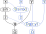
\includegraphics[]{figures/comp-graph}}
  \qquad
  \subbottom[Backward mode.\label{fig:comp-graph-bw}]{%
    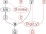
\includegraphics[]{figures/comp-graph-backward}}
  \caption{Computation graph and intermediate expressions of the expression \protect\jlinl{g(sin(x),
      y)}, together with the derivative graphs in forward- and backward mode.  Dashed arrows
    indicate re-use of primal values in the derivative graph.}
  \label{fig:comp-graph-2}
\end{figure}

\newthought{Recovering the full gradient} of a multivariate function
\(\phi: U \subseteq \RR^N \to \RR\) (which is generally the form of loss functions for parametric
models) requires to evaluate \(\Dif \phi(x)\) for \(N\) times.  This is because individual partial
derivatives can only be extracted from \(\Dif \phi(x)\) by calculating the sensitivities to unit
input perturbations in coordinate directions, for each of the input variables:
\begin{equation}
  \nabla \phi(x) = \begin{pmatrix}
    \Dif \phi(x)(1, 0, \ldots, 0)  \\
    \vdots \\
    \Dif \phi(x)(0, \ldots, 0, 1)
  \end{pmatrix} = \begin{pmatrix}
    \partial_1 \phi(x) \\
    \vdots \\
    \partial_N \phi(x)
  \end{pmatrix},
\end{equation}
which is really a special case of taking directional derivatives (which can be recovered generally
by application of the differential to any vector with unit norm.)

In order to overcome the increase of complexity with the number of input dimensions, we can
reformulate the compositional equation.  Let us introduce \(\CoDif \phi(x)\), the \emph{adjoint
  operator} of \(\Dif \phi(x)\), whose defining property is that \enquote{inverts} the order of the
perturbation application: instead of calculating a primal sensitivity with respect to an input
perturbation (\(\Delta\)), it maps a linear output perturbation (\(\mathfrak{d}\)) to an operator
that applies this to the primal sensitivity:
\begin{equation}
  \CoDif \phi(x)(\mathfrak{d}) = \Delta \mapsto \mathfrak{d} \big(\Dif \phi(x)(\Delta) \big).
\end{equation}
The adjoint differential is therefore an object of the double dual space.  This becomes more
readable when we fix a basis to represent the derivative.  Doing so, in the finite-dimensional case,
the derivative \(\Dif \phi(x)\) is the Jacobian matrix at \(x\), \(J_{\phi}(x)\).  In this setting,
forward-mode AD is simply an efficient way to calculate the \emph{Jacobian-vector product}
\(J_{\phi}(x) \Delta\), or equivalently the total derivative for a fixed perturbation, avoiding full
matrix multiplication~-- which is the reason we have to apply it to the basis vectors to get back
the gradient.  Backward mode, on the other hand, calculates the product of the Jacobian with the
operator that should be applied to the result, but does not yet apply it to the input
perturbation~-- therefore, it returns a matrix:
\begin{equation}
  \begin{aligned}
    \mathfrak{d} \big( \Dif \phi(x)(\Delta) \big) &= \transpose{d} J_{\phi}(x) \Delta \\
    &= \transpose{\big( \transpose{J_{\phi}(x)} d \big)} \Delta \\
    &= \CoDif \phi(x)(\mathfrak{d})(\Delta),
  \end{aligned}
\end{equation}
where we assume \(\mathfrak{d}\) to be represented by the co-vector \(\transpose{d}\).  Since the
unapplied \(\CoDif \phi(x)(\mathfrak{d})\) is itself an object in the dual space, it is also
represented as a co-vector~-- and in fact, nothing else than a transformation of the transposed
Jacobian, or a \emph{vector-Jacobian product}.  Recovering the gradient of a loss function then
reduces to evaluating it at a constant scalar output perturbation of \(1\), which is equivalent to
the application of the primal differential to the matrix of basis vectors.

Note that due to this relation to the transpose, the adjoint operator inverses the order of
composition in the chain rule:
\begin{equation}
  \begin{aligned}
    \CoDif (\phi \circ \psi)(x)(\mathfrak{d}) &= \transpose{d} J_{\phi}(\psi(x)) J_{\psi}(x) \\
    &=  \transpose{\big( \transpose{J_{\psi}(x)} \transpose{J_{\phi}(\psi(x))} d \big)} \\
    &= \big( \CoDif\psi(x) \circ \CoDif\phi(\psi(x)) \big)(\mathfrak{d}).
  \end{aligned}
\end{equation}
For our example function \(f\), this gives the same structural form of the result as the forward
mode~-- only that now, the value is a vector:
\begin{equation}
  \begin{aligned}
    \CoDif f(x, y) &= \CoDif \big( g \circ (\sin \otimes \ident) \big)(x, y) \\
    &= \CoDif(\sin \otimes \ident) \circ \CoDif g \big( (\sin \otimes \ident)(x, y) \big) \\
    % &= (\CoDif\sin \otimes \CoDif\ident) \circ (\delta \mapsto \transpose{[\delta, -\delta]}) \\
    % &= (\partial_1 \sin(x) \otimes 1) \circ (\delta \mapsto \transpose{[\delta, -\delta]}) \\
    % &= \delta \mapsto \transpose{[\partial_1\sin(x)\delta, -1 \delta]} \\
    &= \delta \mapsto \transpose{[\cos(x)\delta, -\delta]}.
  \end{aligned}
\end{equation}
In this form, starting with an output perturbation \(\delta = 1\), we get back the complete gradient
vector through just one evaluation.  Incidentally, this is nothing else than the back-propagation
\enquote{trick} \parencite{bishop2006pattern}!  Furthermore, applying this result to
\([\Delta_1, \Delta_2]\) gives back the linear combination of the forward mode result.

In programmatic terms, we can proceed similar to above, only this time introducing \emph{adjoint}
intermediate values \(\bar{v}\).  For the values in equation~\eqref{eq:ad-primal}, we get
\begin{equation}
  \label{eq:ad-backward}
  \begin{aligned}
    \bar{x} &= \bar{z}_2 = -\delta, \\
    \bar{y} &= \CoDif\sin(x) \, \bar{z}_1 \\
    &= \cos(x) \, \delta\\
    \bar{z} &= \CoDif g(x, y)(\bar{\Omega}) \\
    &= [\delta, -\delta] \\
    \bar{\Omega} &= \delta,
  \end{aligned}
\end{equation}
which is displayed in the red graph in \ref{fig:comp-graph-bw}.  Note that now, the back-propagated
values can not be computed in parallel with forward evaluation; hence the equations are stated in
reverse order.  Instead of one lockstep evaluation, the intermediate primal values have to be stored
and reused in a second, backward pass.

Finally, it has to be noted that the two described modes of automatic differentiation are only two
extremes of a spectrum.  Forward and backward calculations can really be interleaved in arbitrary
order, just as it is possible to multiply Jacobians and their transposes in different order.  One
frequent use case of this \emph{mixed-mode AD} is when loss functions, differentiated using backward
mode, contain broadcasting functions, e.g., nonlinearities within neural networks.  These have a
type of \(\RR^N \to \RR^N\), but only involve a linear number of operations, so forward mode pays
off\footnote{As a rule of thumb in Julia, for \(f: \RR^M \to \RR^N\), forward mode typically
  performs better when \(M \ll N\) or as long as \(M \lessapprox 100\).  This folklore should always
  be confirmed by benchmarking, though.  See
  \url{https://github.com/JuliaDiff/ReverseDiff.jl\#should-i-use-reversediff-or-forwarddiff}.}.
Similar properties hold for second order derivatives: the calculation of Hessians is often fastest
by using forward-over-reverse composed differentiation.  In general, unfortunately, determining the
optimal order of derivative evaluation is hard~-- this so-called \emph{optimal Jacobian
  accumulation} problem is known to be NP-complete \parencite{naumann2007optimal}.

\subsection*{Dual Numbers}
\label{sec:dual-numbers}

Forward mode can be recast in mathematically equivalent form by using dual numbers
\parencites[see][section 3.1.1]{baydin2018automatic}{deakin1966functions}.  These consist of two
parts, similar to complex numbers: \(z = x + y\epsilon\).  However, unlike to the imaginary unit,
the infinitesimal unit \(\epsilon\) vanishes under multiplication with itself: \(\epsilon^2 = 0\).
The consequence of this is that analytic functions can naturally be extended to dual numbers by
nonstandard interpretation as truncated Taylor series:
\begin{equation}
  \phi(x + \epsilon) = \phi(x) + \partial_1\phi(x)\epsilon + \underbrace{\frac{\partial^2_1\phi(x)}{2}\epsilon^2
  + \ldots}_{\epsilon^2 (\ldots) = 0}
\end{equation}
Since the higher order terms vanish, this is exactly the tuple of primal and tangent value that is
calculated during the lockstep evaluation in forward mode:
\begin{equation}
  (z, \dot{z}) = (\phi(x), \Dif\phi(x)(\dot{x})) \quad\Leftrightarrow\quad z + \dot{z}\epsilon = \phi(x + \dot{x}\epsilon).
\end{equation}
The generalization to higher dimensions, as well as higher derivatives in form of hyper-dual numbers
\parencite{fike2012automatic}, follow naturally.





%%% Local Variables: 
%%% TeX-master: "main"
%%% End:

% -------------------------------------------------------------------------------
% BACK MATTERN
\cleartorecto
\backmatter
\begingroup
\microtypesetup{protrusion=false, expansion=false}
\raggedright
\phantomsection
\addcontentsline{toc}{chapter}{Bibliography}
\printbibliography[heading=memoir]
\endgroup

%%% Local Variables: 
%%% TeX-master: "main"
%%% End:

% \begingroup
% \hypersetup{hyperindex=true}
% \listofalgorithms
% \endgroup



% \chapter{Example Programs}
% \label{sec:appendix}


% -------------------------------------------------------------------------------
% COLOPHON
\cleartoverso
\thispagestyle{empty}
\renewcommand{\abstractname}{Colophon}
\begin{abstract}
  \noindent
  This document was typeset using the pdf\LaTeX{} typesetting system, with the memoir document
  class. The body text is set in 11\,pt Linux Libertine, enhanced by the microtype package. Other
  fonts include Biolinum and Inconsolata.
  % The drawings are typeset using
  % TikZ/PGF, and source code examples are formatted by the listings package.

  The document source has been written in Emacs with AUC\TeX{} mode, using TeXworks as \abbrev{PDF}
  viewer.  Figures were created in Inkscape, and plotting done in R using ggplot2.
\end{abstract}

%%% Local Variables:
%%% mode: latex
%%% TeX-master: "main"
%%% End:

\end{document}

%%% Local Variables: 
%%% TeX-master: "main"
%%% mode: latex
%%% TeX-command-extra-options: "-shell-escape"
%%% End:
